% This is samplepaper.tex, a sample chapter demonstrating the
% LLNCS macro package for Springer Computer Science proceedings;
% Version 2.20 of 2017/10/04
%
\documentclass[runningheads]{llncs}
%
\usepackage{graphicx}
% Used for displaying a sample figure. If possible, figure files should
% be included in EPS format.
%
\usepackage{color}
\usepackage{hyperref}
\usepackage{subfigure}
\newcommand{\threeimage}[6]{
\begin{figure}[h!]
    \centering
    \subfigure[]{
        \includegraphics[width=0.25\linewidth, height=0.25\linewidth]{#1}
        \label{fig_f_ #1} }
        %\hspace{4ex}
    \subfigure[]{
    \includegraphics[width=0.25\linewidth, height=0.25\linewidth]{#2}
    \label{fig_f_ #2} }
   % \hspace{4ex}
    \subfigure[]{
        \includegraphics[width=0.25\linewidth, height=0.25\linewidth]{#3}
        \label{fig_f_ #3} }
    \caption{
    \subref{fig_f_ #1} #4;
    \subref{fig_f_ #2} #5;
    \subref{fig_f_ #3} #6}
    \label{fig:f_ #1#2#3}
\end{figure}}

% If you use the hyperref package, please uncomment the following line
% to display URLs in blue roman font according to Springer's eBook style:
\graphicspath{{img/}}
\renewcommand\UrlFont{\color{blue}\rmfamily}

\begin{document}
%
\title{Plant Seedlings Classification}
% If the paper title is too long for the running head, you can set
% an abbreviated paper title here
%
\author{Dmitri Jakovlev \and Julia Kamaletdinova \and Georgy Shevlyakov}
% \author{First Author\inst{1}\orcidID{0000-1111-2222-3333} \and
% Second Author\inst{2,3}\orcidID{1111-2222-3333-4444} \and
% Third Author\inst{3}\orcidID{2222--3333-4444-5555}}
%
\authorrunning{D. Jakovlev, J. Kamaletdinova et al.}
% First names are abbreviated in the running head.
% If there are more than two authors, 'et al.' is used.
%
\institute{Peter the Great Saint-Petersburg Polytechnic University, Department of Applied Mathematics, Russia}

% \institute{Princeton University, Princeton NJ 08544, USA \and
% Springer Heidelberg, Tiergartenstr. 17, 69121 Heidelberg, Germany
% \email{lncs@springer.com}\\
% \url{http://www.springer.com/gp/computer-science/lncs} \and
% ABC Institute, Rupert-Karls-University Heidelberg, Heidelberg, Germany\\
% \email{\{abc,lncs\}@uni-heidelberg.de}}
%
\maketitle              % typeset the header of the contribution
%
\begin{abstract}
The abstract should briefly summarize the contents of the paper in
150--250 words.

\keywords{First keyword  \and Second keyword \and Another keyword.}
\end{abstract}
%
%
%

%!TEX root = paper.tex
\section{Introduction}
%\indent{\indent The need for agricultural products is %increasing every day, as the population of planet %Earth is growing. Part of the work is done by people, %and the forces go to quality control of crops grown. %We will be able to use temporary and natural resources %more carefully and economically, increase yields if we %learn to differentiate noble crops and distinguish %them from weeds without human help. }

\indent{\indent The demand for agricultural products is increasing day by day, as the population of the Earth is growing. Even though people are working on plant classification algorithms, approaches are still not as robust as desired. A significant part of work has still been done by people. The question arises of the efficiency with which human resources are used. We will use exhaustible natural resources wisely and increase harvests if we will automatise quality assurance, which objectives are to detect and distinguish weeds among the variety of crop seedlings.}

\indent{ All this naturally leads to idea of automation of the classification process with help of machine learning algorithms. From recent experience, neural networks are well suited for image processing, but we have to pay for it with computational costs. On the other hand, we could use less costly algorithms, but they require finer tuning to achieve a comparable result.}

\indent{ The goal is to implement segmentation and classification of a specific type of data set for low time and computational complexity. In this paper we will research binary classifiers capabilities on the dataset \cite{giselsson2017public} consisting of images of 12 species and containing the most common weed species in Danish agriculture.}


%!TEX root = paper.tex
\section{Materials and methods}
%!TEX root = paper.tex
\subsection{Data}

\indent{\indent The considered dataset is a part of the database that has been recorded at the Aarhus University Flakkebjerg Research station in the collaboration between the University of Southern Denmark and Aarhus University. Images are available to researchers at \url{https://vision.eng.au.dk/plant-seedlings-dataset/}. The specifics of this dataset is that recorded plants are in different growth stages since detecting a weed in its early stage is the thing which makes the task problematic. }

\indent{The dataset contains 960 unique plant images of 12 species. The sizes of plant classes are not balanced among themselves---they range from 221 to 654 labeled samples for each class. Original images are cropped by plant boundaries, but their resolutions vary from 50x50px to 2000x2000px. Also, images have  different backgrounds---some of them are on the ground, other are on the marked paper.}

\begin{figure}[h]
    \centering
    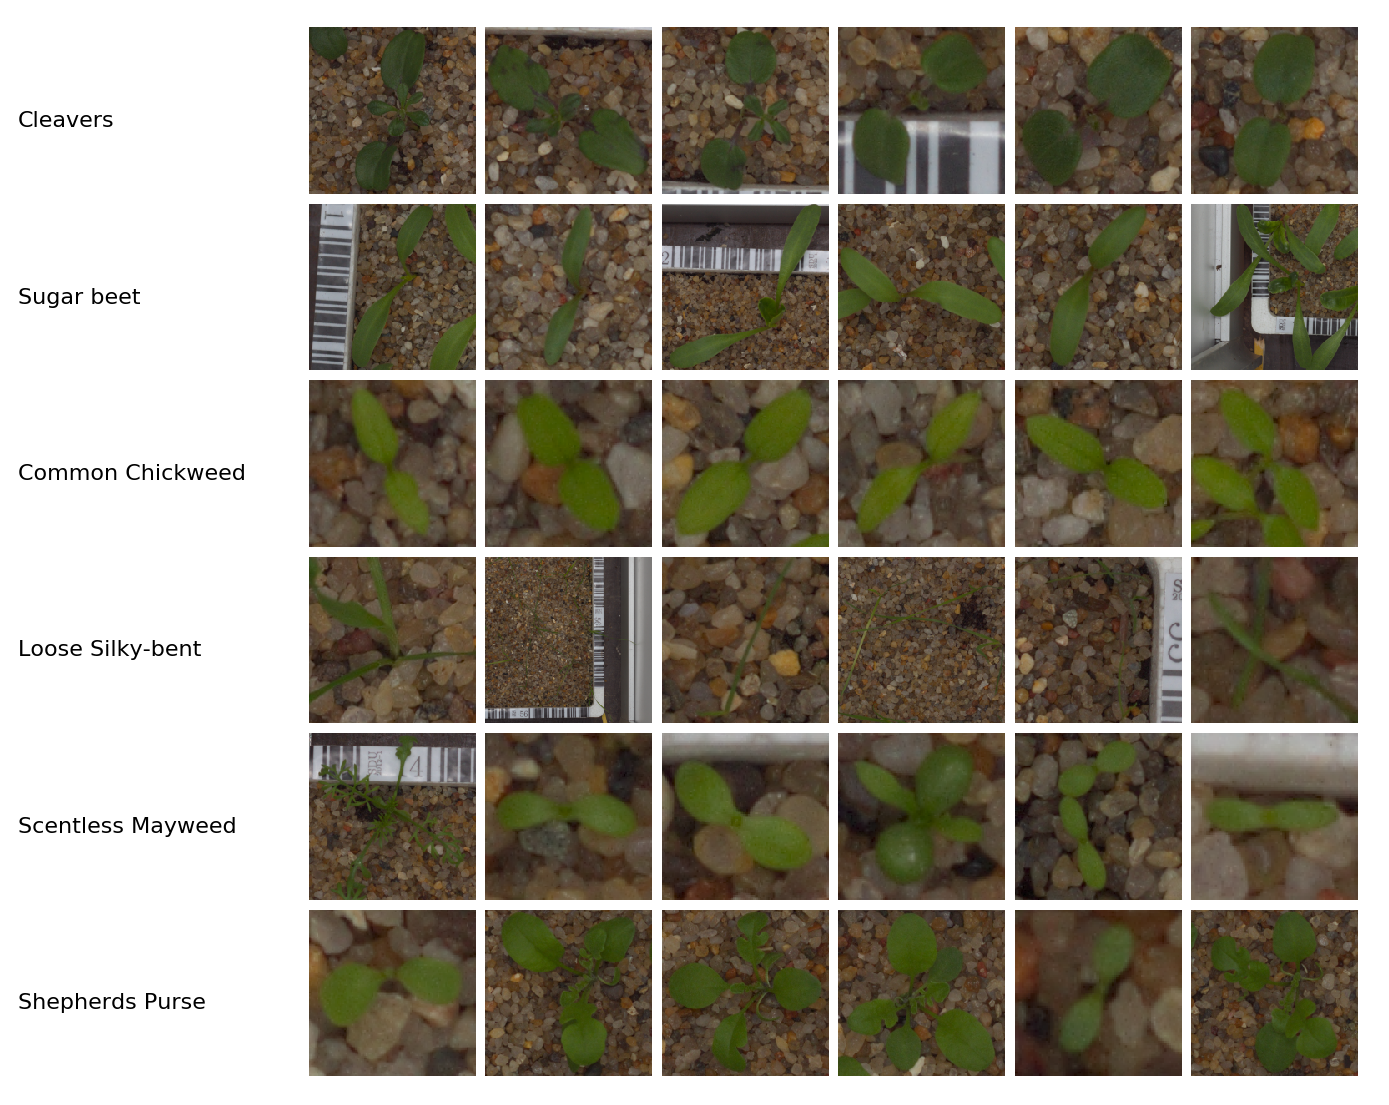
\includegraphics[height=8.5cm, width=10.5cm]{first_view_grid_smaller_1}
    \caption{Data overview}
    \label{fig:1}
\end{figure}

\subsection{Data preprocessing}
\indent{\indent \textbf{Resolution reducing}}

\indent{\indent \textbf{Resolution reducing}}\quad {We reduce the resolution of all images to the same resolution 200x200px using the bilinear interpolation. The main idea of the bilinear interpolation is that a new image pixel is defined as the weighted sum of neighboring pixels of the original image. It helps to decrease computational complexity and build normalized features \cite{bilinear1963interp}.}

\textbf{Segmentation} \quad {The objects of our study are plants, and they are painted green. Therefore, we can create a mask that filters the range of green channel and ignores the other pixels. For these purposes, the HSV (Hue Saturation Value) color model is a suitable representation \cite{hsv1978color}. In the BGR (Blue Green Red) format, the value of each component depends on the amount of light hitting the object. HSV allows us to distinguish between the image color and brightness. We set the lower and upper bounds of the green color using HSV representation. Then we merely mark the pixels in the green range and get a color mask (Fig. \ref{fig_f_ seg_step_2}). Now we apply the operation of logical multiplication to the original image, assign the value of the background pixels to a black color value, and get a segmented plant.}

\threeimage{seg_step_1}{seg_step_2}{seg_step_3}{Source image}{Mask}{Segmented image}

\textbf{Denoising}\quad {Segmentation does not always work well (see Fig. \ref{fig_f_ seg_step_3}). Small areas of the background may fall into the range of green values which distorts the binary mask as in Fig. \ref{fig:seg_no_morph_1}}.

\begin{figure}[h]
	\centering
    \subfigure[Before morphological closure]{
		{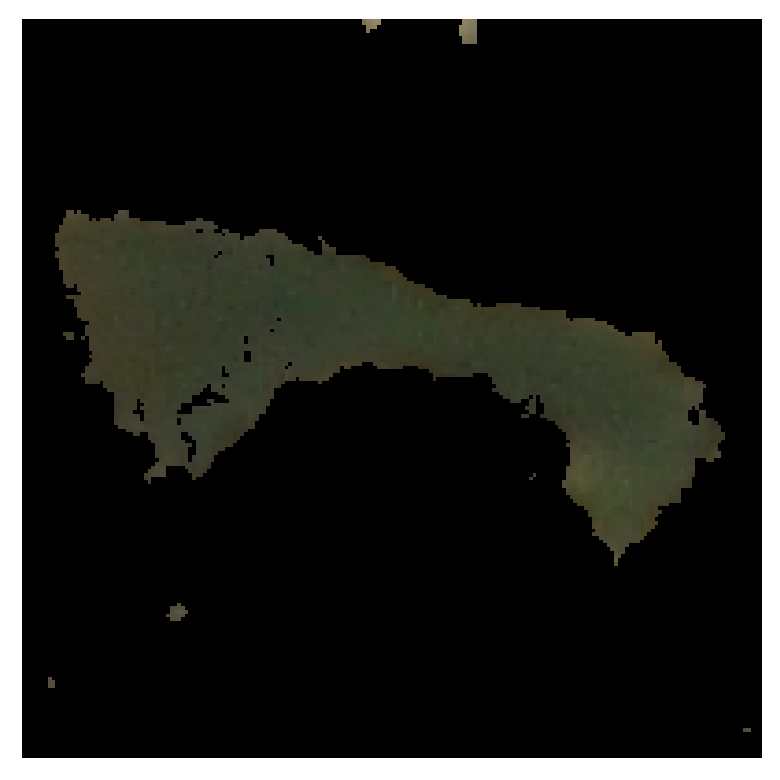
\includegraphics[width=5cm, height=5cm]{seg_no_morph_1}
		\label{fig:seg_no_morph_1}}
	}
    \qquad
    \subfigure[After morphological closure]{
		{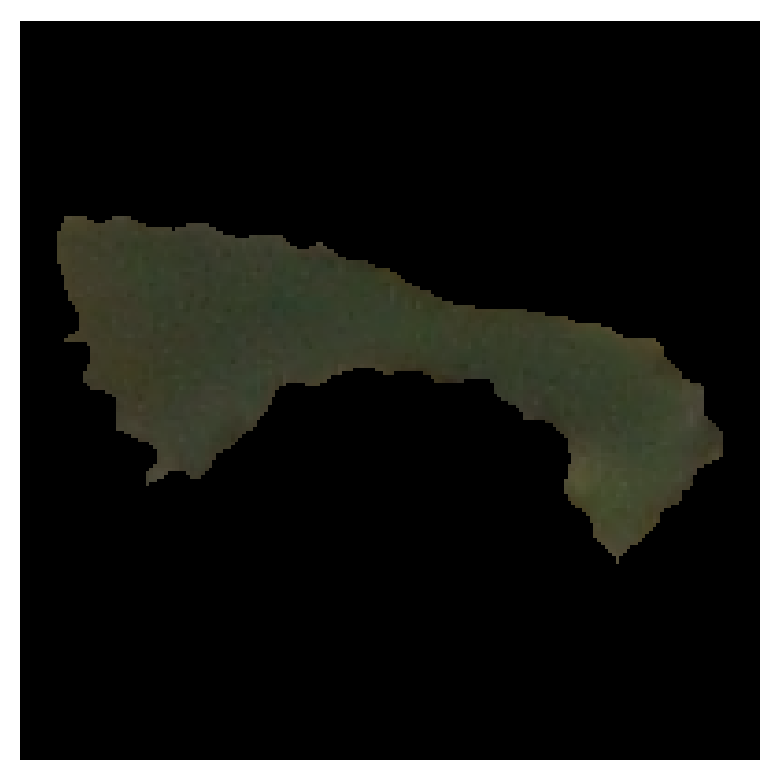
\includegraphics[width=5cm, height=5cm]{seg_morph_1}
		\label{seg_morph_1}}
	}
    \caption{Segmentation improvement example}%
    \label{fig:seg_improve}
\end{figure}

\indent{Such drawbacks can be eliminated by the morphological operations of the nonlinear transformation associated with the shape and structure of an image. The morphology is used to study the interaction of an image with a specific structural element,  \emph{the kernel}. The kernel iterates over the entire image and compares the neighborhoods of pixels after which we apply morphological operations \cite{friel2000imanalysis}.}

\indent{To improve segmentation, we use the operation of the morphological closure---a combination of the dilatation and erosion operations \cite{morph2000java}.}

\indent{Then we apply the morphological closure operation to the image (Fig. \ref{fig:seg_no_closure_good_1}) by selecting an elliptical core of 6x6px size and delete the remaining objects within an area of less than 160px. The plant on the image (Fig. \ref{fig:seg_with_closure_bad_1}) has no cavities, and the background is cleared of non-plant elements. But the morphological closure does not always improve the segmentation result. Estimate the result of processing an image of the class Loose silky-bent in Fig. \ref{fig:seg_degradation}: the cavities corresponding to the background were restored that does not correspond to the desired result. We restrict ourselves to the removal of objects whose contours limit a small area.}

\begin{figure}[h]
	\centering
    \subfigure[Before morphological closure]{
		{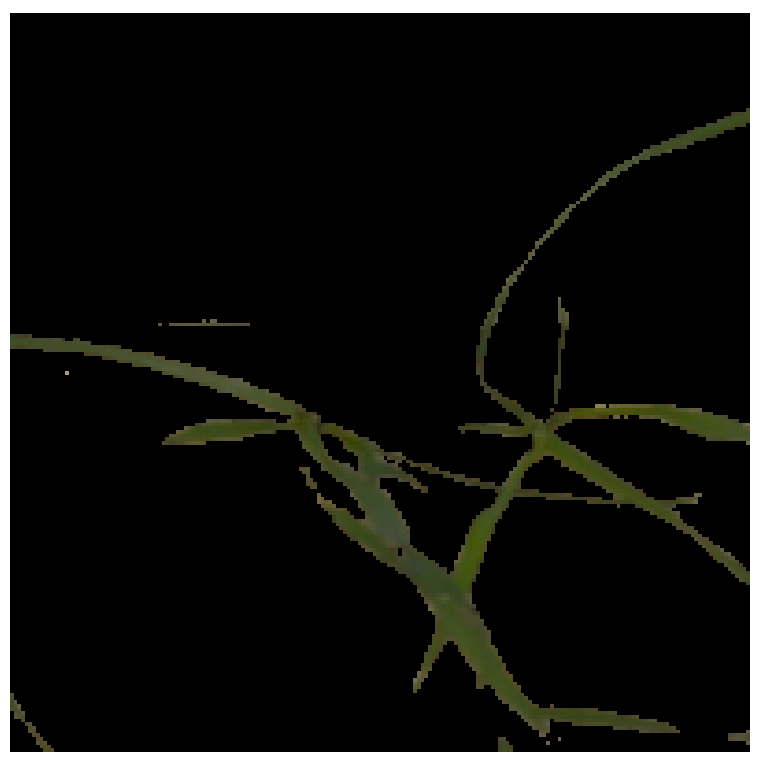
\includegraphics[width=5cm, height=5cm]{seg_no_closure_good_1}
		\label{fig:seg_no_closure_good_1}}
	}
    \qquad
    \subfigure[After morphological closure]{
		{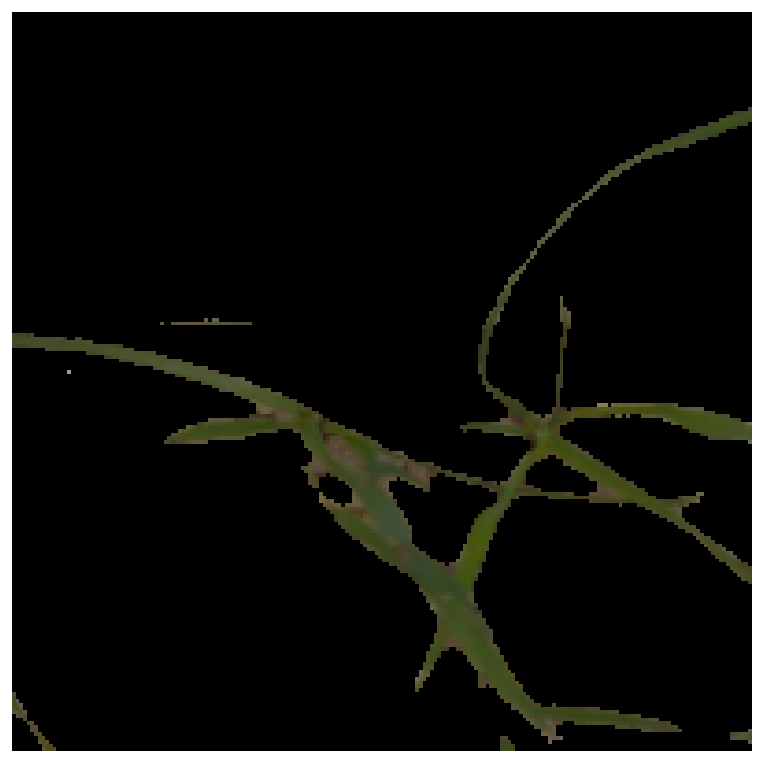
\includegraphics[width=5cm, height=5cm]{seg_with_closure_bad_1}
		\label{fig:seg_with_closure_bad_1}}
	}
    \caption{Segmentation degradation example}%
    \label{fig:seg_degradation}
\end{figure}


\subsection{Feature selection}

\indent{\indent The features of images define their content. Consideration of a great number of features helps us to recognize the information better. Image features let the classifier propose the output decision. Another advantage of the approach is that it reduces feature space for a machine learning algorithm. We often need only a part of the information on the image, hence we do not need to process and evaluate all the pixels, which can cause additional computational expenses.}

\indent{ Selecting features is a complicated and convoluted research area itself, the statement is supported by the variety of feature types, and the need of presenting essential properties on an equal basis with the previous assertion.}

\indent{The goal is to define the set of features describing the dataset in the best way. Supposed features must satisfy the following criteria:}

\begin{enumerate}
    \item The feature space should be low-dimensional
    \item The features should not correlate or correlate as little as possible
    \item Selected features should represent the content of an image as fully as possible
\end{enumerate}

\indent{ Now we are going to define the selected features.}

\subsection{Color features}

\indent{\indent Overviewing the dataset, we notice that all the plant species are mostly green. Additionally, their images are recorded under specific conditions. We use the RGB color model, which stands for red, green, and blue colors, and calculate features described below.}

\begin{figure}[h]
    \centering
    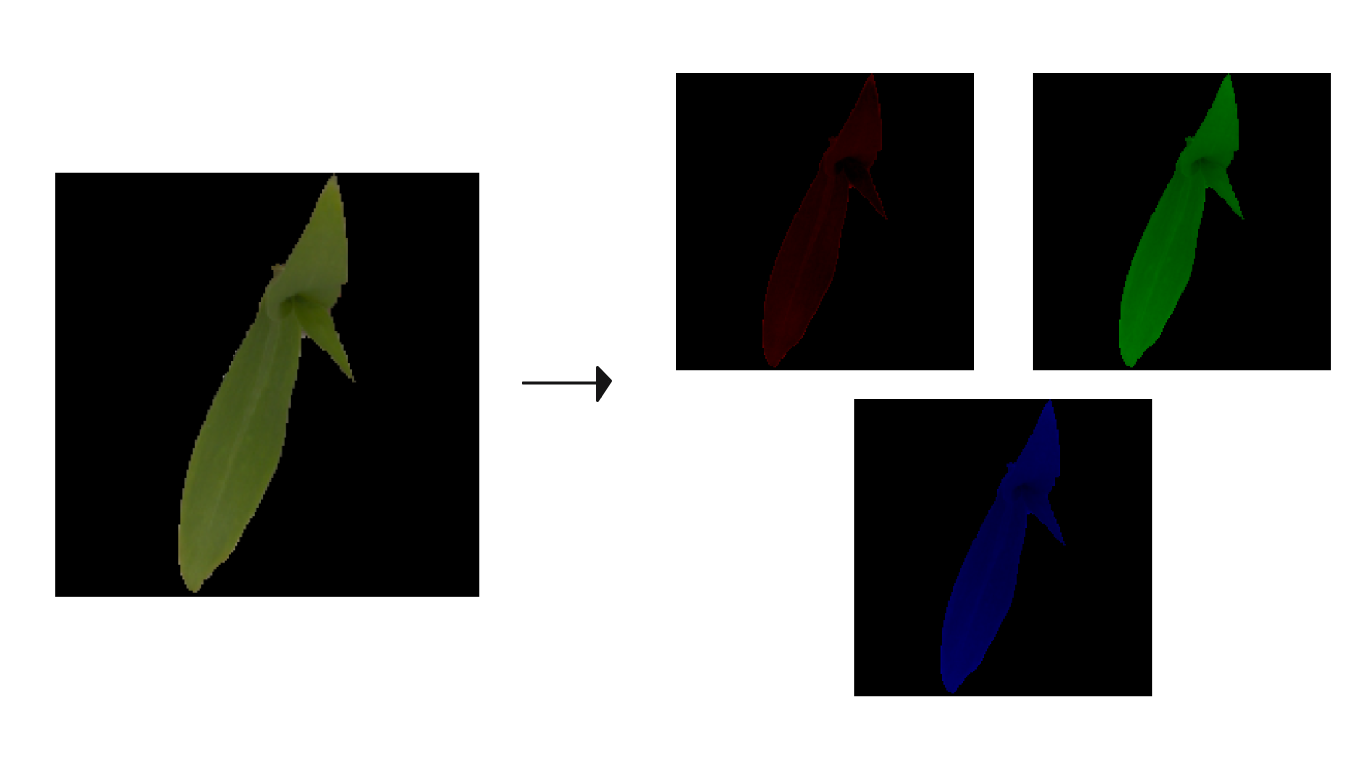
\includegraphics[height=5.5cm, width=10cm]{to_rgb_sample_1}
    \caption{RGB transformation}
    \label{fig:2}
\end{figure}

\indent{Let $\{x^{(k)}\}_{i=1}^N$, where $k = 1, 2, 3 $ is an index of a channel in the RGB color space, respectively; $N$ is a total number of the image pixels; $x^{(k)}_i$ is an $i$-th pixel of the $k$-th channel. Next, compute the sample mean and standard deviation for each channel:}

\begin{equation}
	\label{eq:1}
	\overline{x^{(k)}} = \frac{1}{N}\sum_{i=1}^{N}x^{(k)}_i,
\end{equation}

\begin{equation}
	\label{eq:2}
	 s^{(k)} = \sqrt{\frac{1}{N}\sum_{i=1}^{N}(x^{(k)}_i - \overline{x^{(k)}})^2}.
\end{equation}

\subsection{Shape features}

\indent{\indent A widely-used approach to retrieve shape features is to detect and analyze bounding contours. Here we use the boundary tracing algorithm for the boundary extraction. The designated algorithm \cite{cv1985contours} is implemented in the OpenCV \cite{opencv2000python} library for the Python programming language. The studies do not take into account the contours bounding areas below a certain threshold, which is empirically chosen.}

\indent{ Let $K$ be a number of detected bounding contours above the threshold in the further contour-related characteristics.}

\vspace{1cm}

\textbf{Total perimeter}. For this feature, we count the sum of perimeters of all the areas bounded by contours:

\begin{equation}
	\label{eq:3}
	 P = \sum_{i=1}^{K}p_i,
\end{equation}
where $p_i$ is an $i$-th perimeter.

\vspace{1cm}

\textbf{Entire area}. It includes all the areas bounded by contours:

\begin{equation}
	\label{eq:4}
	 S = \sum_{i=1}^{K}s_i,
\end{equation}
where $s_i$ is an $i$-th area.

\vspace{1cm}

\textbf{Maximal contour area}. Here, we analyze the contours bounding maximal areas:

\begin{equation}
	\label{eq:5}
	 S_m = \max{s_i}, \; i = 1, \dots, K.
\end{equation}


\vspace{1cm}

\textbf{Rectangularity}. One of the methods to estimate rectangularity is to plot minimum bounding rectangle. Rectangularity is the ratio of the entire object area to the minimum bounding rectangle area. This feature represents how rectangular an object is:

\begin{equation}
	f_{rect} = \frac{S}{S_{MBR}},
	\label{eq:6}
\end{equation}
where $S$ is the entire area, $S_{MBR}$ is the minimum bounding rectangle area.

\vspace{1cm}

\textbf{Circularity}. Another title of this shape factor is the isoperimetric quotient, and it shows how much area per perimeter is bounded:

\begin{equation}
	f_{circ} = \frac{4 \pi A}{P^2},
	\label{eq:7}
\end{equation}
where $P$ is an entire perimeter; $A$ is an entire area of all detected elements of a plant.

\indent{ The correlation matrix of the described features has the form:}

\begin{figure}[h]
	\centering
	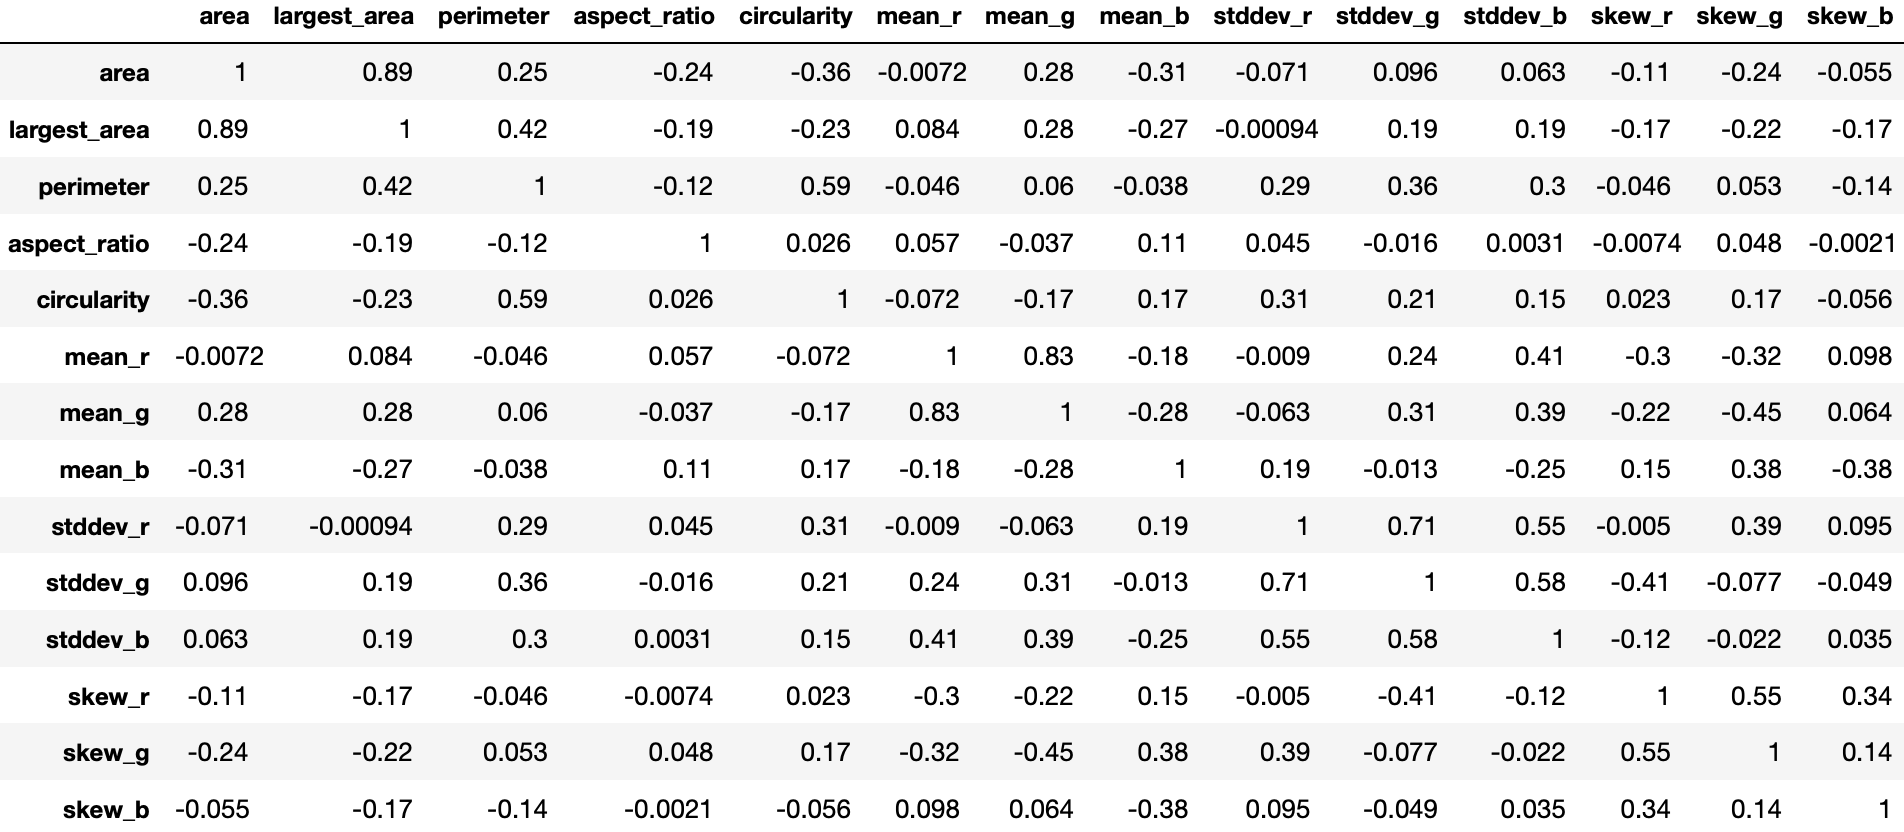
\includegraphics[width=12.cm, height=5.5cm]{corr_matrix_plain}
	\caption{Feature correlation matrix}
	\label{fig_corr_matrix}
\end{figure}

\indent{ Based on the data in Fig. \ref{fig_corr_matrix}, we conclude that the most linearly dependent features are the entire area and the largest area. This is not true for all classes due to the predominance of plants bounded by the only one contour. Therefore, the largest area feature is not rejected.}

\subsection{Classification}
\indent{\indent The main method for solving this task is the Support Vector Machine (SVM) \cite{svmguide2003article}, a binary classification algorithm based on building a separating hyperplane. The other methods we apply are the K-Nearest Neighbors \cite{k2007nearest}, Naive Bayes \cite{naive2001bayes} and Decision Tree \cite{breiman1984classification} classifiers. These algorithms are implemented in the Scikit-learn (\cite{scikit2011python}) library for the Python programming language.}

\indent{ We use the Radial Basis Function (RBF) as the kernel function for SVM. This choice is made because the RBF allows to build a hyperplane when the data is not linearly separable. }


\textbf{Data normalization}. The SVM algorithm is sensitive to non-normalized data, especially when using the RBF kernel, which is just the Euclidian distance. In the case when the feature values are at different intervals, a slight difference in one of them can lead to going out of range in second feature values. The solution is to map all the values into one segment. In this task, we choose the segment $[0, 1]$.


%!TEX root = paper.tex
\section{Results}
\subsection{Metric}

\indent{\indent Results of classification are evaluated on a micro-averaged F-score. Given the positive and negative rates for each class, the resulting score is computed the following way:}

\begin{equation}
    Precision_{micro} = \frac{\sum_{k \in C} TP_k}{\sum_{k \in C} TP_k + FP_k}, \;\;
    Recall_{micro} = \frac{\sum_{k \in C} TP_k}{\sum_{k \in C} TP_k + FN_k}
    \label{eq:PR}
\end{equation}

\begin{equation}
    F_{micro} = \frac{2*Precision_{micro}*Recall_{micro}}{Precision_{micro} + Recall_{micro}},
    \label{eq:mic_f1}
\end{equation}
where $C$ –– set of the plants classes

\vspace{1cm}

\indent{ The choice of such a metric is supported by the fact that classes are imbalanced. In this case, the influence of classes decreases due to averaging by classification characteristics, not by F-scores.}

\indent{The classificator result is shown in the table \ref{table:metrics}}. \\

\begin{table}[h!]
    \caption{Detailed metrics for SVM classificator}
    \begin{center}
        \begin{tabular}{lccc}
            \toprule
            \textbf{Type} & \textbf{Precision} & \textbf{Recall} & \textbf{F-score} \\
            \midrule
            Sugar beet       & 0.901 & 0.936 & 0.918 \\
            Fat Hen          & 0.877 & 0.909 & 0.893 \\
            Scentless Mayweed & 0.851 & 0.905 & 0.878 \\
            Charlock         & 0.947 & 0.934 & 0.940  \\
            Small-flowered Cranesbill & 0.963 & 0.991 & 0.977 \\
            Maize            & 0.953 & 0.891 & 0.921   \\
            Shepherds Purse  & 0.833 & 0.714 & 0.769 \\
            Common Wheat     & 0.800 & 0.889 & 0.842 \\
            Common Chickweed & 0.962 & 0.962 & 0.962 \\
            Cleavers         & 0.885 & 0.852 & 0.868 \\
            Loose Silky-bent & 0.828 & 0.888 & 0.857  \\
            Black-grass      & 0.757 & 0.528 & 0.622 \\
            \midrule
            \multicolumn{3}{l}{Micro-averaged F-score} 0.885 \\
            \bottomrule
            \label{table:metrics}
        \end{tabular}
    \end{center}
\end{table}

\subsection{Models comparison}

\indent{\indent The choice of the SVM is justified by better results in comparison with other classical methods of machine learning. Table \ref{table:metrics_all} shows micro-averaged F-scores for Naive Bayes, k-nearest neighbours and Decision tree classifiers. The methods are implemented in Scikit-learn (\cite{scikit2011python}) library. All the experiments were conducted 100 times each, on shuffled data, the metrics were obtained by testing on a validation sample and averaged.}

\begin{table}[h!]
    \caption{Metrics for used classificators}
    \begin{center}
        \begin{tabular}{lc}
            \toprule
            \textbf{Method} & \textbf{Micro-averaged F-score} \\
            \midrule
            naiveBayes & 0.72 \\
            kNN & 0.84 \\
            decisionTree & 0.73 \\
            \textbf{SVM} & \textbf{0.885} \\
            \bottomrule
            \label{table:metrics_all}
        \end{tabular}
    \end{center}
\end{table}


%!TEX root = paper.tex
\section{Discussion}


%!TEX root = paper.tex
\section{Conclusion}


\section{Acknowledgments?}
% ---- Bibliography ----
%
% BibTeX users should specify bibliography style 'splncs04'.
% References will then be sorted and formatted in the correct style.
%
\bibliographystyle{splncs04}
\bibliography{mybibliography}


\end{document}
